\section{Auswertung}
\label{sec:Auswertung}

\subsection{Fehlerrechnung}
\label{sec:Fehlerrechnung}
Für die Fehlerrechnung werden folgende Formeln aus der Vorlesung verwendet.
für den Mittelwert gilt
\begin{equation}
    \overline{x}=\frac{1}{N}\sum_{i=1}^N x_i ß\; \;\text{mit der Anzahl N und den Messwerten x} 
    \label{eqn:Mittelwert}
\end{equation}
Der Fehler für den Mittelwert lässt sich gemäß
\begin{equation}
    \increment \overline{x}=\frac{1}{\sqrt{N}}\sqrt{\frac{1}{N-1}\sum_{i=1}^N(x_i-\overline{x})^2}
    \label{eqn:FehlerMittelwert}
\end{equation}
berechnen.
Wenn im weiteren Verlauf der Berechnung mit der fehlerhaften Größe gerechnet wird, kann der Fehler der folgenden Größe
mittels Gaußscher Fehlerfortpflanzung berechnet werden. Die Formel hierfür ist
\begin{equation}
    \increment f= \sqrt{\sum_{i=1}^N\left(\frac{\partial f}{\partial x_i}\right)^2\cdot(\increment x_i)^2}.
    \label{eqn:GaussMittelwert}
\end{equation}

\subsection{Bestimmung der Grenzspannung}
\label{sec:Auswertunga}

Zur Bestimmung der Grenzspannung $U_{\text{g}}$ wird eine Ausgleichsgerade durch die Messwerte gelegte. Hierbei ist zu beachten, dass die Ausgleichsgerade die linearen Abschnitte der hauptsächlich Bremsspannung umfasst.
Die Nullstelle dieser Geraden ist dann die gesuchte Spannung. Für $U_{\text{g}}$ folgt somit
\begin{equation}
    U_{\text{g}}=-a/b\, .
    \label{eqn:U_g}
\end{equation}

Die in \autoref{fig:rot} dargestellten Messwerte mit der dazugehörigen Ausgleichsgeraden liefern die Funktionsparameter 
\begin{align*}
    a_{\text{rot}}&=(4.18\pm 0.33) \, \unit{\frac{\ampere ^{1/2}}{\volt}}\\
    b_{\text{rot}}&=(3.41\pm 0.06) \, \unit{\ampere}^{1/2}\, .\\
\end{align*}
Draus folgt gemäß \autoref{eqn:U_g} ein Wert von $U_{\text{g,rot}}=(-0.82\pm 0.07)\, \unit{\volt}$.
\begin{figure}
    \centering
    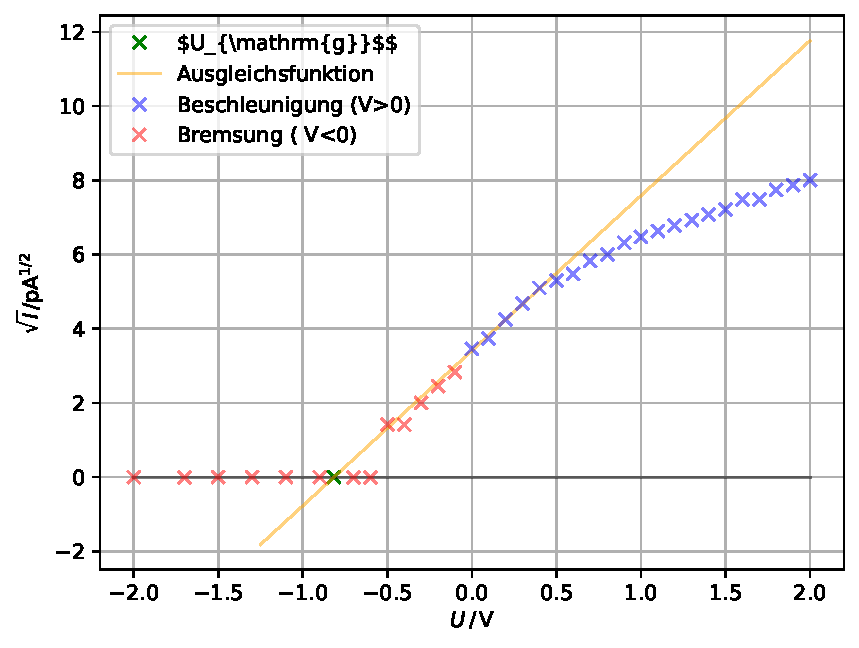
\includegraphics[height = 8cm]{build/plotrot.pdf}
    \caption{Regression zur Bestimmung der Grenzspannung $U_{\symup{g}}$ der roten Spektrallinie.}
    \label{fig:rot}
\end{figure}
Anlog zur Bestimmung von $U_{\text{g}}$ des roten Lichtes wurde die Grenzspannung der anderen beiden Wellenlängen 
berechnet.
Die Messwerte und Ausgleichsgerade des grünen Lichtes ist in \autoref{fig:gruen} aufgetragen.
\begin{align*}
    a_{\text{grün}}&=(34.50\pm 1.40) \, \unit{\frac{\ampere ^{1/2}}{\volt}}\\
    b_{\text{grün}}&=(23.90\pm 0.50) \, \unit{\ampere}^{1/2}\, .\\
    \Rightarrow U_{\text{g,grün}}&=(-0.69\pm 0.03)\, \unit{\volt}\\
\end{align*}

\begin{figure}
    \centering
    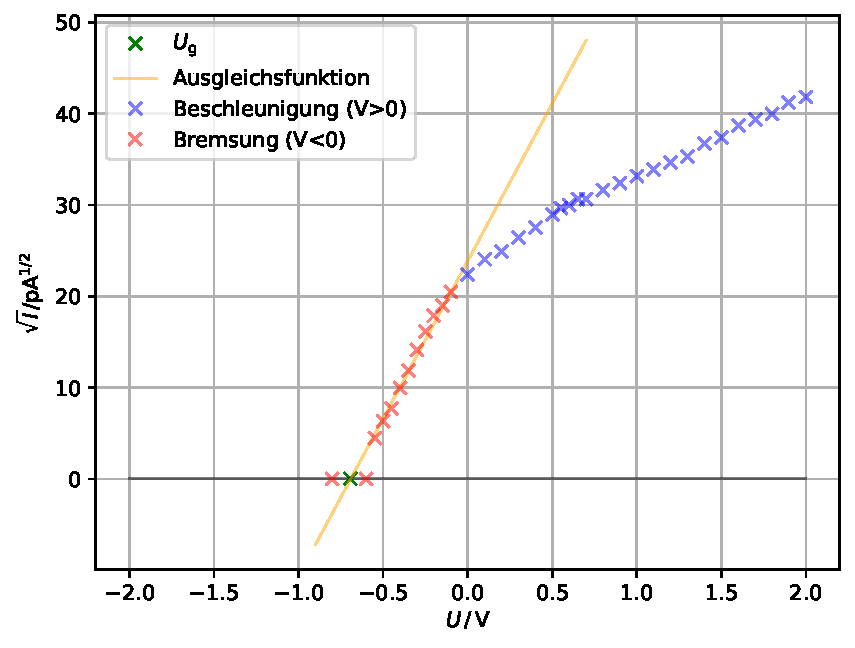
\includegraphics[height = 8cm]{build/plotgruen.pdf}
    \caption{Regression zur Bestimmung der Grenzspannung $U_{\symup{g}}$ der grünen Spektrallinie.}
    \label{fig:gruen}
\end{figure}

Die Messwerte und Ausgleichsgerade des grünen Lichtes ist in \autoref{fig:lila} aufgetragen.
\begin{align*}
    a_{\text{lila}}&=(0.80\pm 0.030) \, \unit{\frac{\ampere ^{1/2}}{\volt}}\\
    b_{\text{lila}}&=(0.98\pm 0.01) \, \unit{\ampere}^{1/2}\, .\\
    \Rightarrow U_{\text{g,lila}}&=(-1.22\pm 0.04)\, \unit{\volt}\\
\end{align*}

\begin{figure}
    \centering
    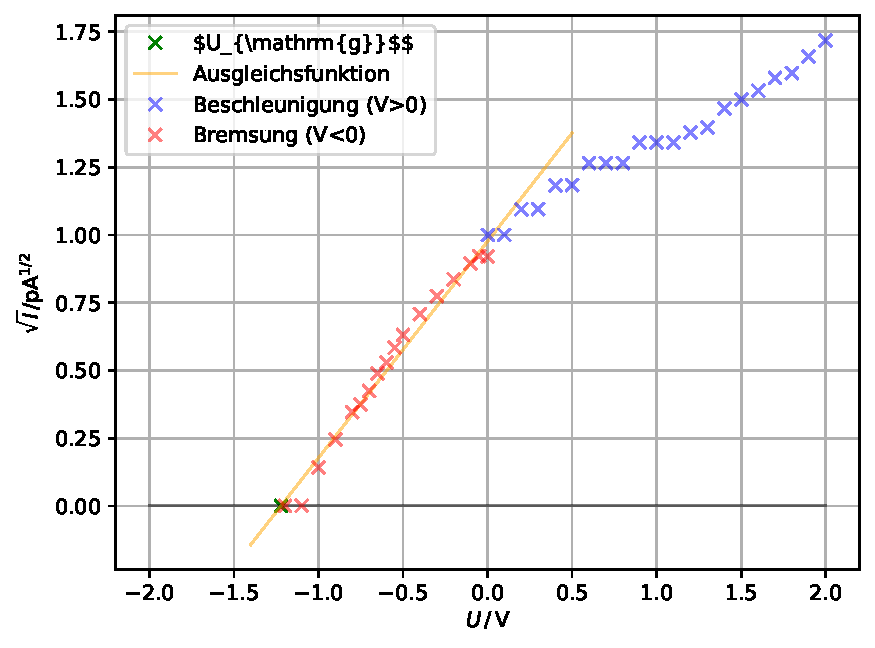
\includegraphics[height = 8cm]{build/plotlila.pdf}
    \caption{Regression zur Bestimmung der Grenzspannung $U_{\symup{g}}$ der violetten Spektrallinie.}
    \label{fig:lila}
\end{figure}

\begin{figure}
    \centering
    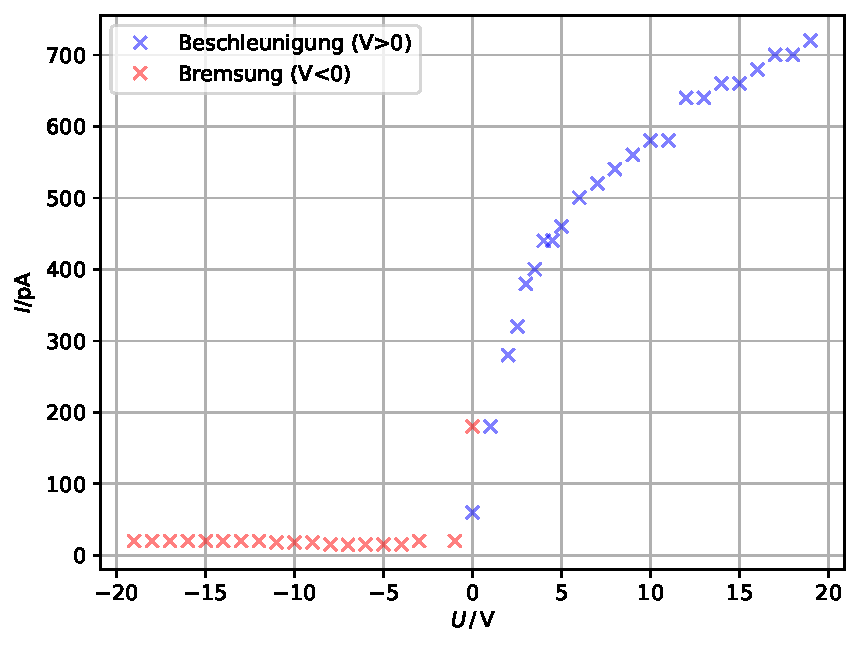
\includegraphics[height = 8cm]{build/plotgelb.pdf}
    \caption{Verlauf des Photostroms der gelben Spektrallinie bei $\lambda = 578 \,\unit{\nm}$.}
    \label{fig:gelb}
\end{figure}

